\chapter{Popis použitých technologií a testovacího prostředí}

\section{OpenStack}\label{sub:interaction}

Popis Openstacku

\subsection{Heat Templates}

Popis co jsou to heat templates.

Heat is the main project of the OpenStack orchestration program. It allows users to describe deployments of complex cloud applications in text files called templates. These templates are then parsed and executed by the Heat engine.

\begin{figure}[h]
\begin{centering}
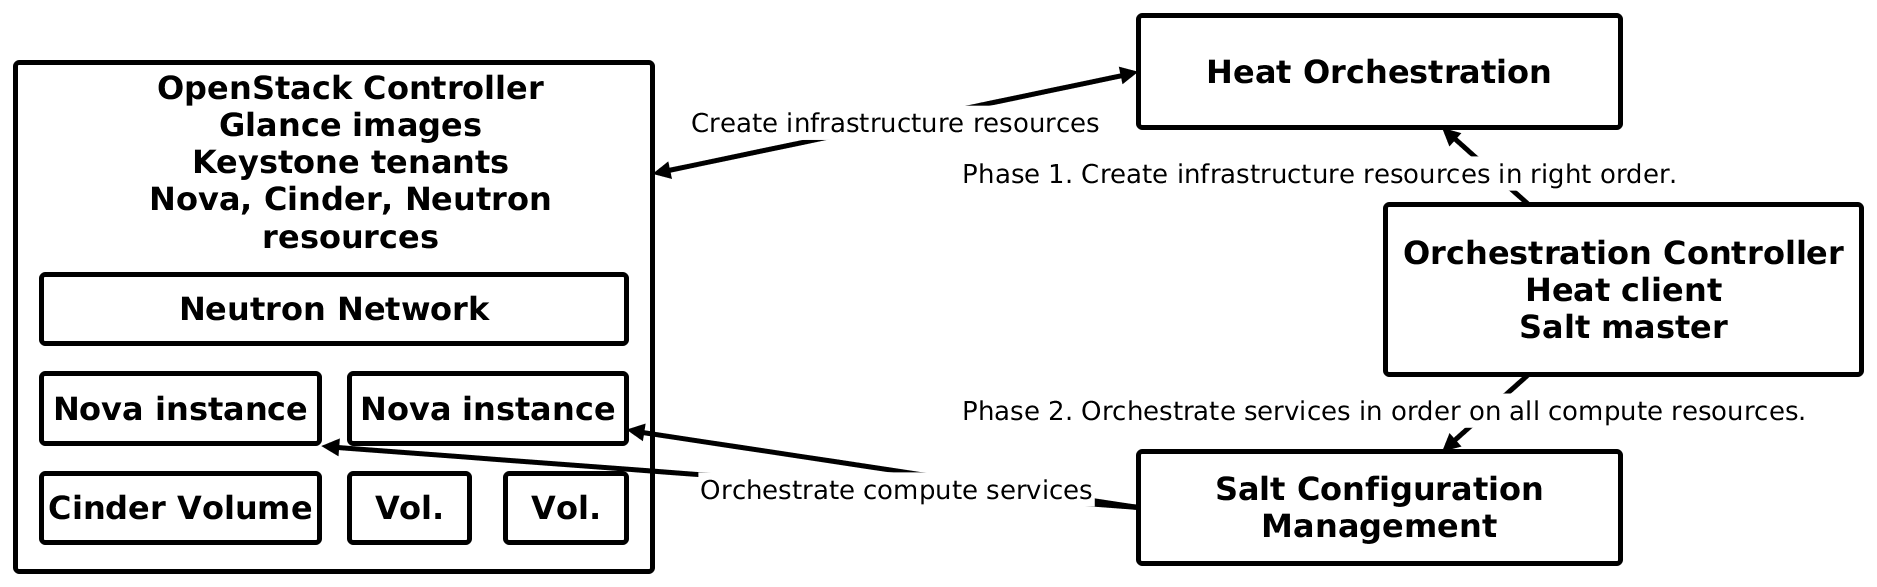
\includegraphics[scale=0.21]{images/heat}
\par\end{centering}
\caption{Popis heat orchestrace\label{fig:heat}}
\end{figure}

OpenStack Heat Templates are used to demonstrate load balancing and firewalling inside of Openstack.

\section{OpenContrail}\label{sub:interaction}

Popis OpenContrailu.

\subsection{Service Chaining}

Popis service chaining v contrail a service instanci.
a jak to může být využito pro VNF.


\section{Testovací topologie}\label{sub:interaction}

The NFV topology consist of 5 nodes. The management node is used for public IP access and is accessible via SSH. It is also used as a JUMP host to connect to all other nodes in the blueprint. The controller node is the brains of the operation and is where Openstack and OpenContrail are installed. Finally, we have three compute nodes named Compute 1, Compute 2 and Compute 3 with Nova Compute and the Opencontrail vRouter agent installed. This is where the data plane forwarding will be carried out.

The diagram below display the 5 components used in the topology. All nodes apart from the management node have 8 CPU, 16GB of RAM and 64GB of total storage. The management node has 4 CPU, 4GB of RAM and 32GB of total storage.

\begin{figure}[h]
\begin{centering}
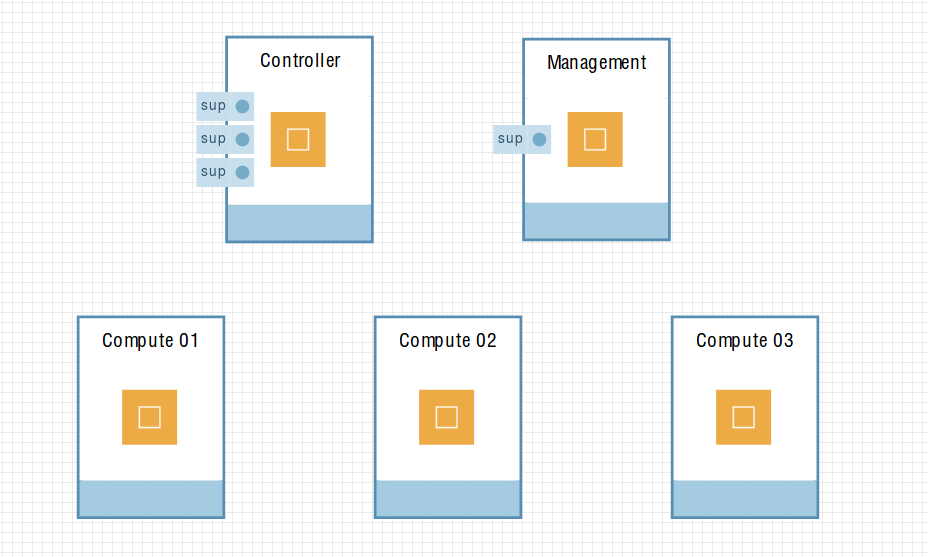
\includegraphics[scale=0.41]{images/ravello_topologie}
\par\end{centering}
\caption{Testovací topologie\label{fig:ravello_topologie}}
\end{figure}


\section{Testované síťové funkce}\label{sub:interaction}

Navrhnutá řešení v této práci předvádějí virtuální víťové funkce pro firewall a load balancing. Jsou zde ukázány celkem 3 scénáře případu užíti. Dva jsou zaměřeny na FwaaS (Firewall as a Service) a jeden na LbaaS (Load balancer as a Service). Všechna řešení jsou vytvořena pomocí Heat templatů, které se spouští v prostředí OpenStack.

Aby mohla být nějaká VNF vůbec vytvořena, tak musel být nejprve zvolen software či operační systěm, který má požadovanou funkci implementovánu. Pro tyto účely byly použity následující řešení:

\begin{itemize}
\item PFSense – open-souce firewall založený na operačním systému FreeBSD.
\item FortiGate-VM – je plnohodnotně vybavený Fortigate firewall zabalený jako virtualní instance.
\item Neutron Agent-HAproxy – je velmi rychlé a spolehlivé řešení nabízející vysokou dostupnost, load balancing a proxy pro aplikace založené na TCP a HTTP
\end{itemize}